\subsection*{NVMe Form Factors}

A form factor is the physical size, shape, and connector design of a hardware device. For an NVMe SSD, the form factor determines 
how the drive fits into a computer and connects to the motherboard, but it does not determine its performance.

NVMe SSDs are available in different form factors, each designed for specific applications and system requirements. The most common 
form factors are M.2, U.2, and Add-in Card (AIC).

\begin{enumerate}
    \item \textbf{M.2:} A compact SSD that connects directly to the motherboard through an M.2 slot. It is widely used in laptops and d
    esktop computers due to its small size and cable-free installation.

    \item \textbf{U.2:} A 2.5-inch enterprise SSD that connects through a U.2 connector using the PCIe interface. It provides high storage 
    capacity and is commonly used in servers and data centers.

    \item \textbf{Add-in Card (AIC):} An NVMe SSD mounted on a PCIe expansion card. It plugs directly into a PCIe slot and offers excellent 
    cooling and high performance, making it suitable for workstations and enterprise systems.\cite{lexar_nvme}
\end{enumerate}

\begin{figure}[H]
    \centering

    \begin{subfigure}{0.3\textwidth}
        \centering
        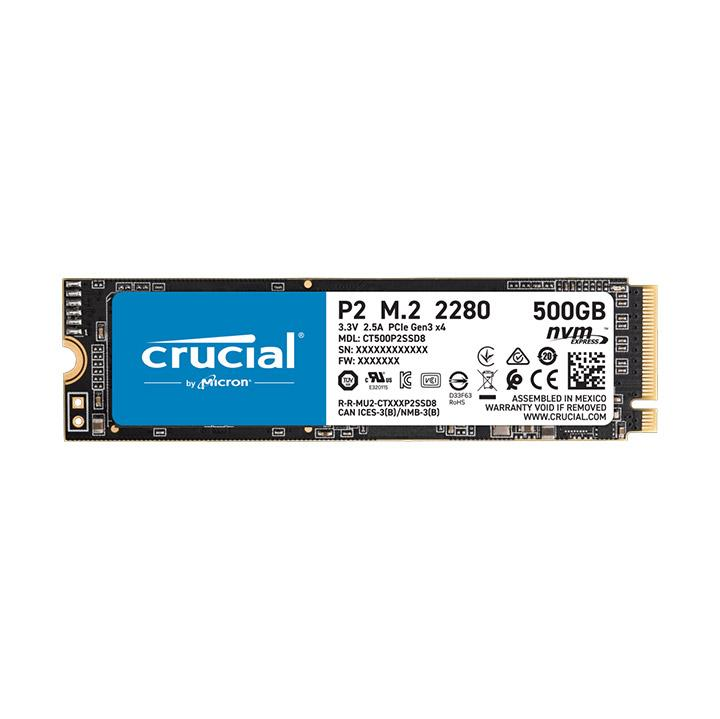
\includegraphics[width=\linewidth]{M.2.jpg}
        \caption{M.2}
    \end{subfigure}
    \hfill
    \begin{subfigure}{0.3\textwidth}
        \centering
        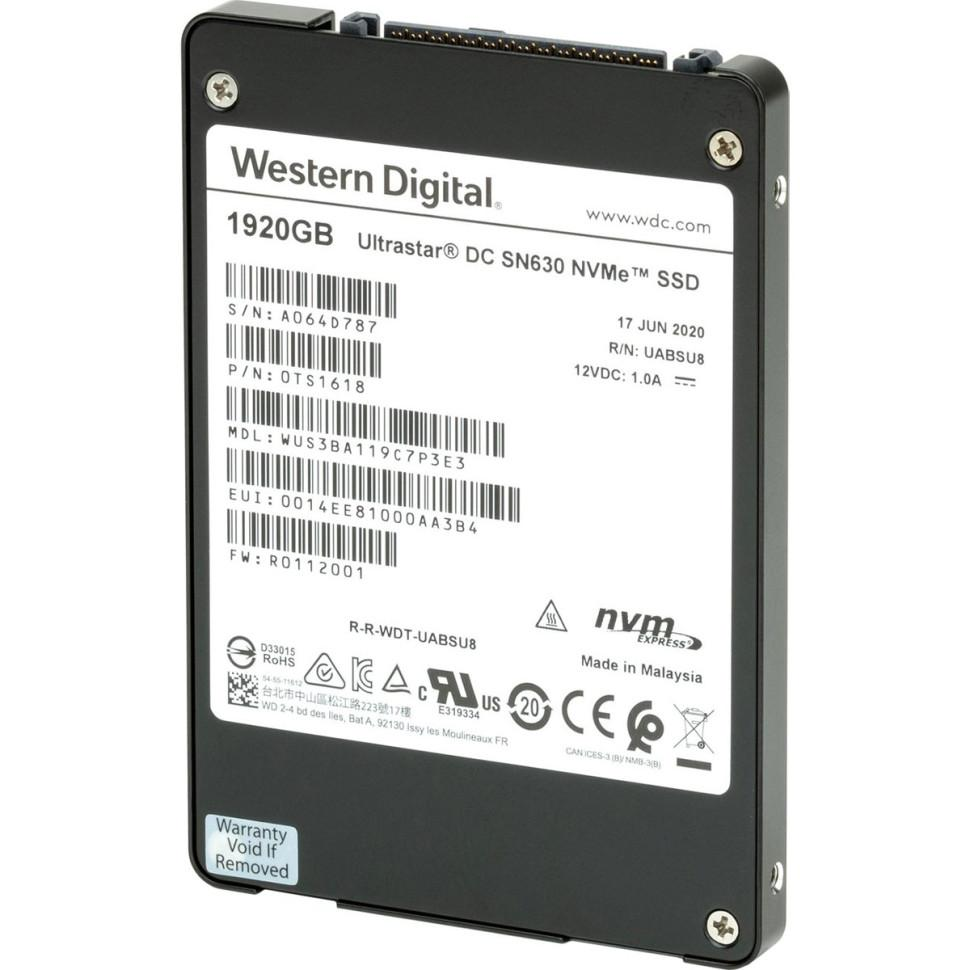
\includegraphics[width=\linewidth]{u.2.png}
        \caption{U.2}
    \end{subfigure}
    \hfill
    \begin{subfigure}{0.3\textwidth}
        \centering
        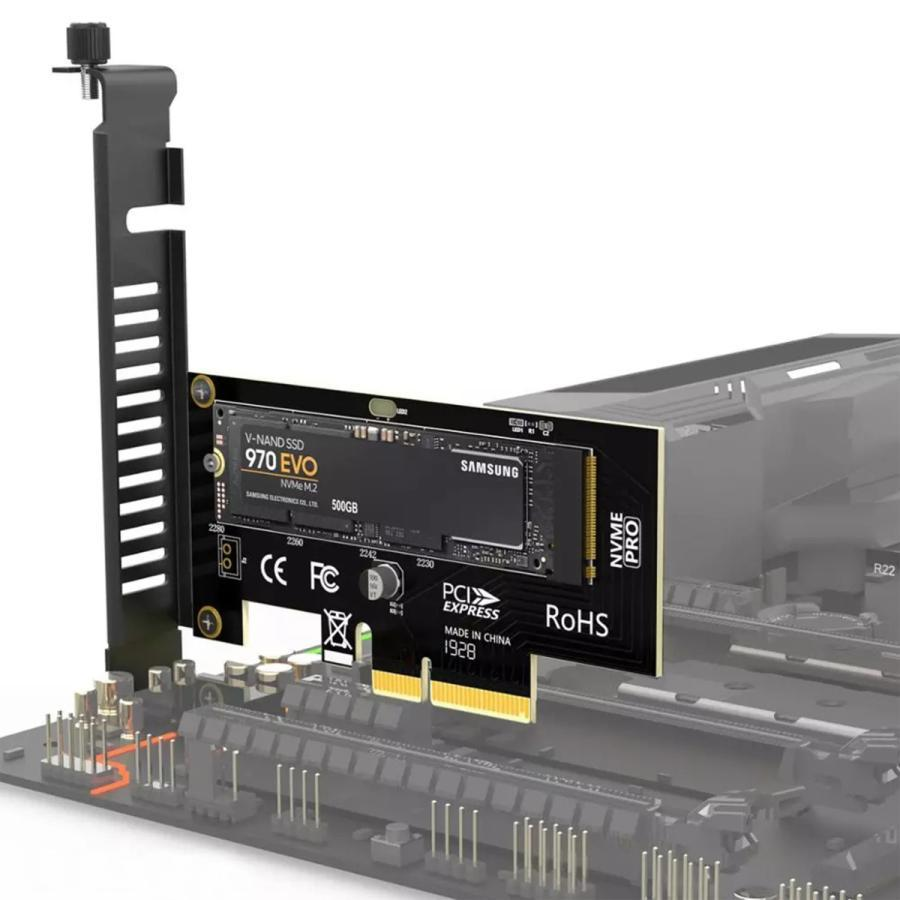
\includegraphics[width=\linewidth]{adi.jpg}
        \caption{Add-in Card (AIC)}
    \end{subfigure}

    \caption{Common NVMe SSD Form Factors}
    \label{fig:nvme_form_factors}
\end{figure}
\newpage
\begin{figure}[H]
    \centering
    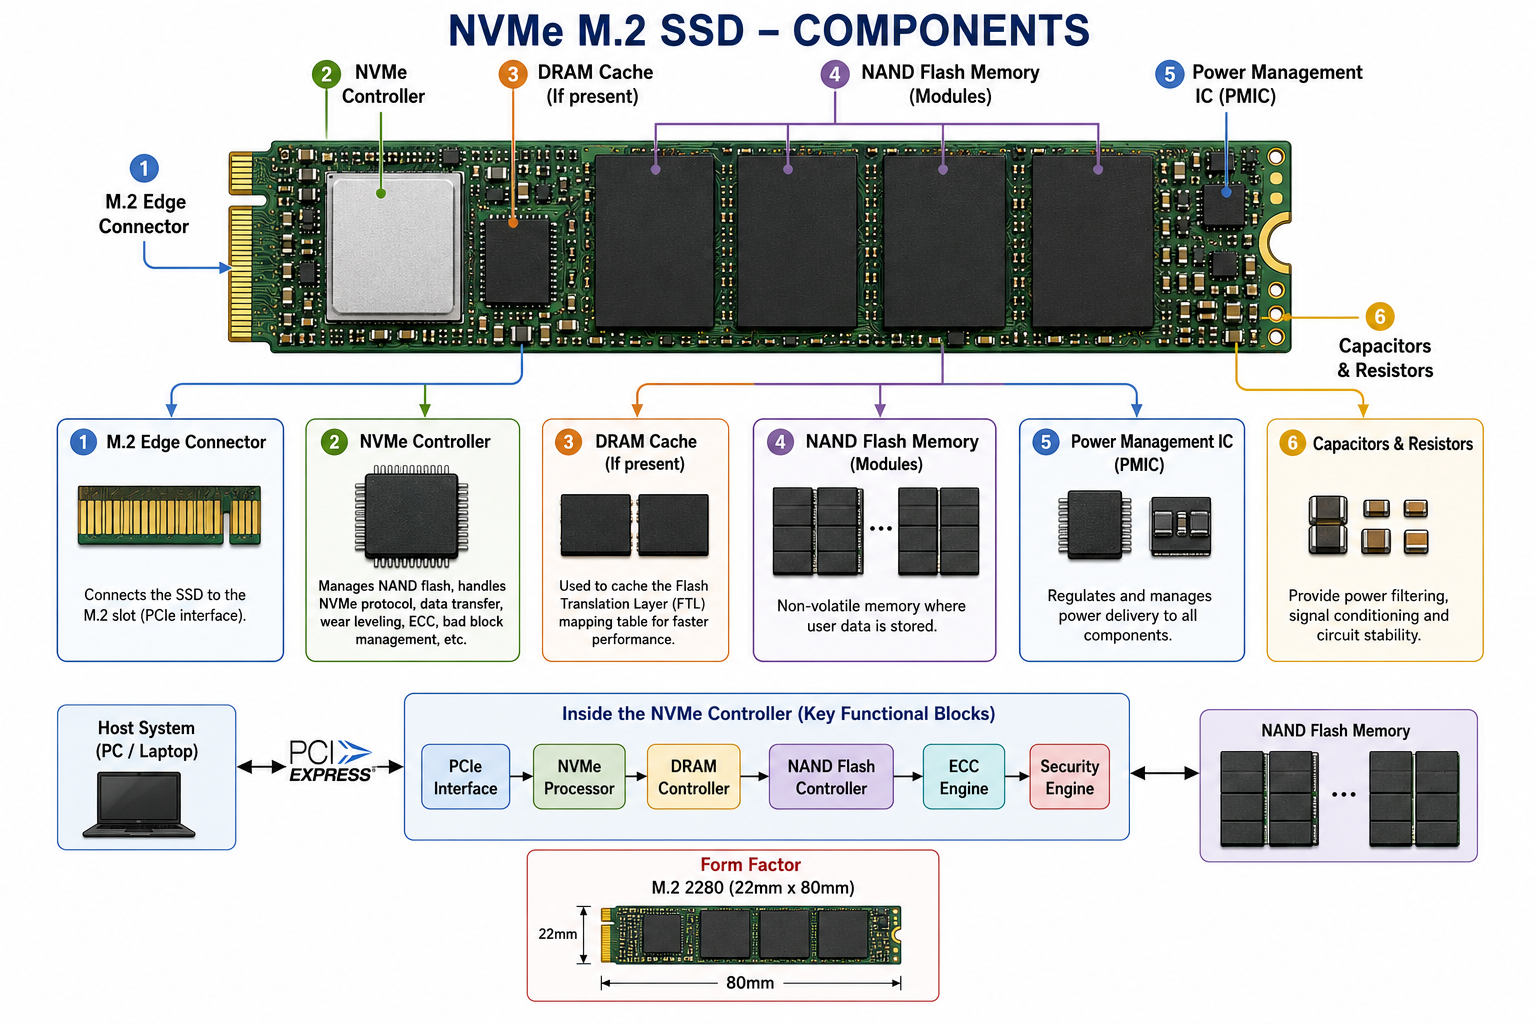
\includegraphics[width=0.9\textwidth]{components of nvme.png}
    \caption{Components of an NVMe SSD}
    \cite{image_generated_nvme}
    \label{fig:nvme}
\end{figure}


\begin{figure}[H]
    \centering
     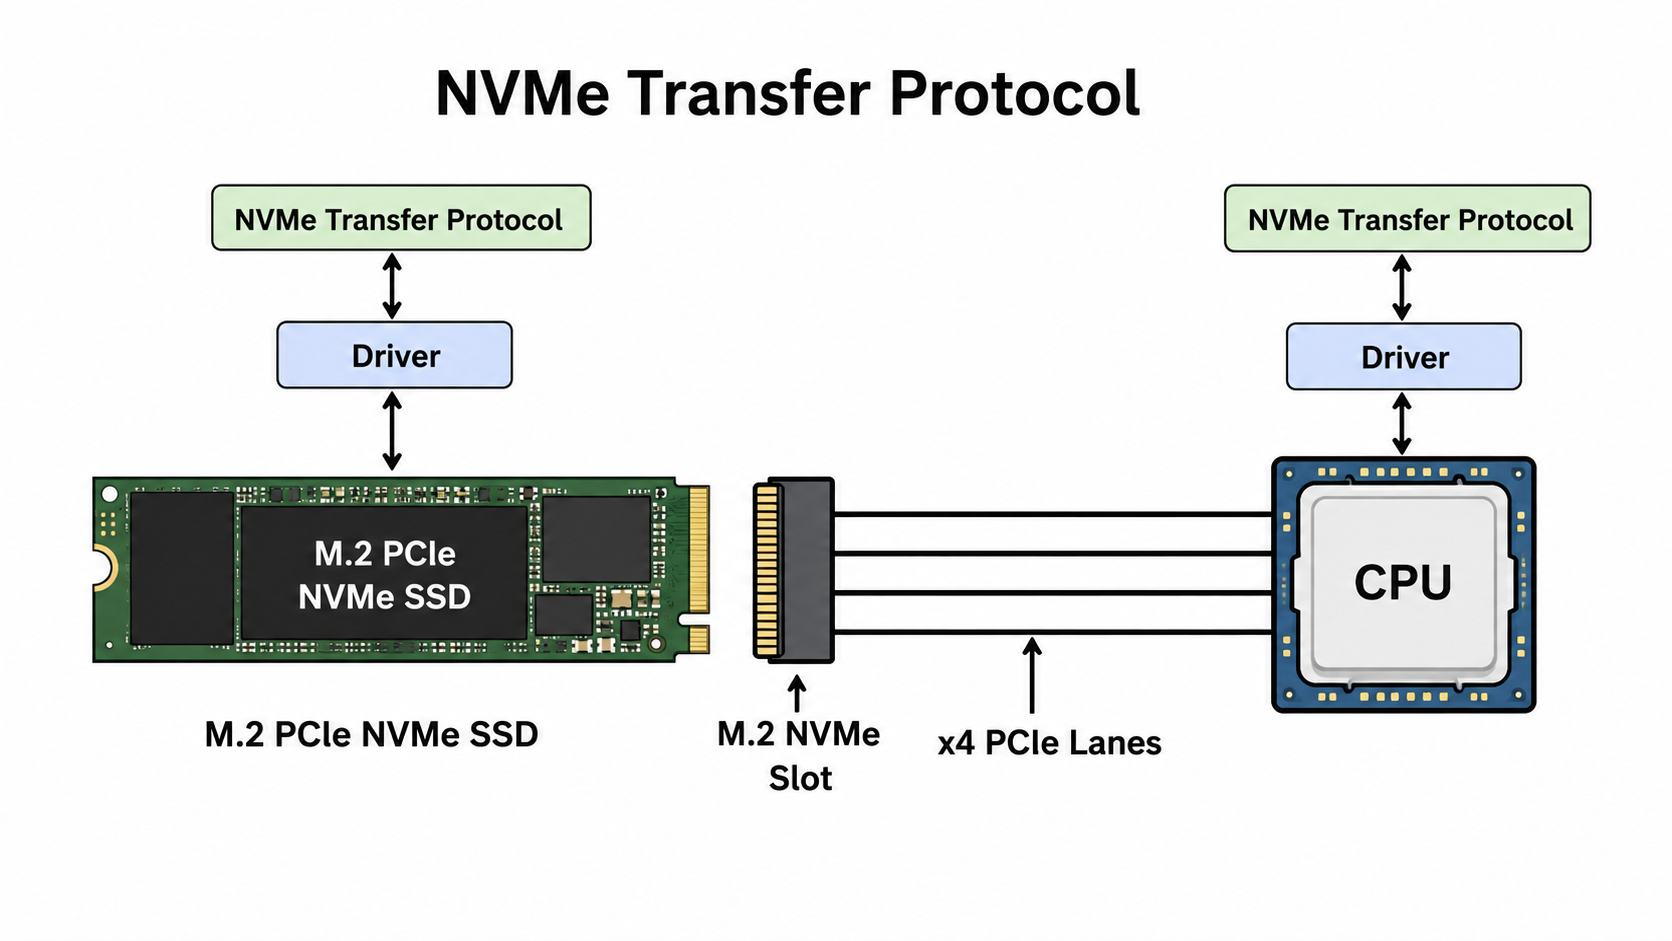
\includegraphics[width=1\textwidth]{NVMe Working.png}
    \caption{NVMe SSD Data Transfer Architecture}
    \cite{nvme_protocol}
    \label{fig:working of nvme}
\end{figure}